\begin{table}
\centering
\caption[Selected inputs for scientific sparse tensor workloads.]{Inputs for the scientific sparse tensor workloads. The table lists SuiteSparse matrices for sparse linear algebra kernels and FROSTT tensors for sparse tensor kernels, along with nonzero counts, dimensions, domains, and matrix-structure visualizations. These inputs span different sparsity patterns and domains, stressing traversal, lookup, and merging in different ways.}
\label{tab:tmu-scientific-inputs}
\resizebox{\columnwidth}{!}{%
\begin{tabular}{@{}cccccc@{}}
\toprule
\textbf{Id} & \textbf{Matrix~\cite{davis2011university}} & \textbf{nnzs} & \textbf{rows} & \textbf{nnzs/row} & \textbf{Domain}\\
\midrule
M1 & af\_0\_k101 & 17.6M & 504K & $\sim$35 & structural  \\
M2 & atmosmodm & 10.3M & 1.5M & $\sim$7     & fluid dynamic  \\
M3 & Freescale1 & 17.1M & 3.4M & $\sim$5    & circuit simulation \\
M4 & gb\_osm & 13.3M & 7.7M & $\sim$2   & graph  \\
M5 & halfb & 12.4M & 225K & $\sim$55         & structural  \\
M6 & test1 & 9.4M & 393K & $\sim$24          & semiconductor  \\
\hline
\textbf{Id} & \textbf{Tensor~\cite{smith2017frostt}} & \textbf{nnzs} & \multicolumn{2}{c}{\textbf{Dimensions}} & \textbf{Domain} \\
\hline
T1 & Chicago-crime & 5M & \multicolumn{2}{c}{6K x 24 x 77 x 32} & count\\
T2 & LBNL-network & 2M & \multicolumn{2}{c}{2K x 4K x 2K x 4K x 1M} & network \\
T3 & NIPS pubs & 3M & \multicolumn{2}{c}{3K x 3K x 14K x 17} & text \\
T4 & Uber pickups & 3M & \multicolumn{2}{c}{183 x 24 x 1K x 2K} & map\\
\hline
\textbf{M1} & \textbf{M2} & \textbf{M3} & \textbf{M4} & \textbf{M5} & \textbf{M6} \\ 
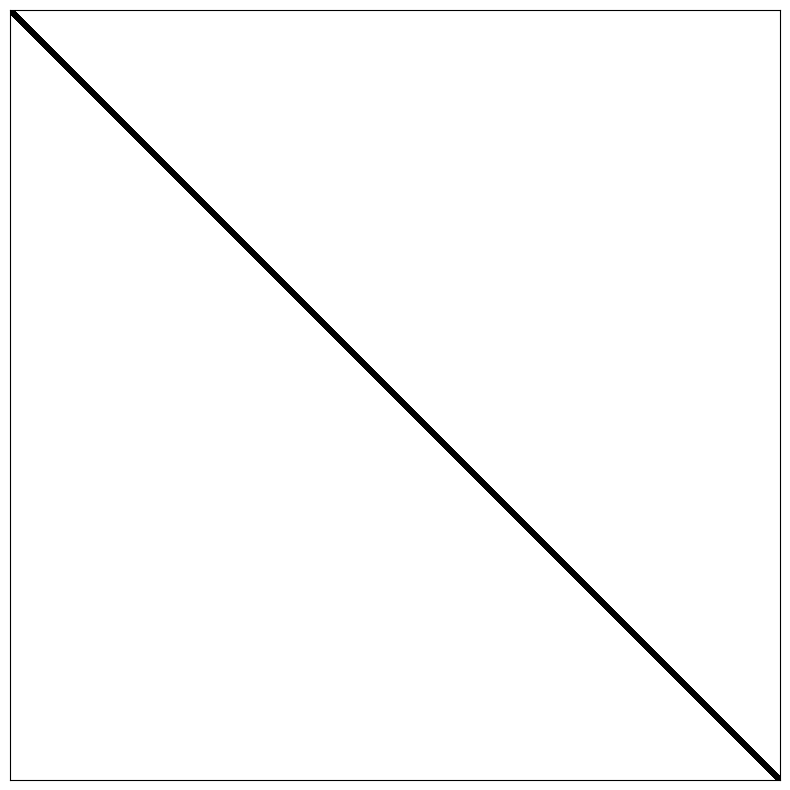
\includegraphics[width=.2\linewidth]{img_mtx_af_0_k101-crop.png}  &
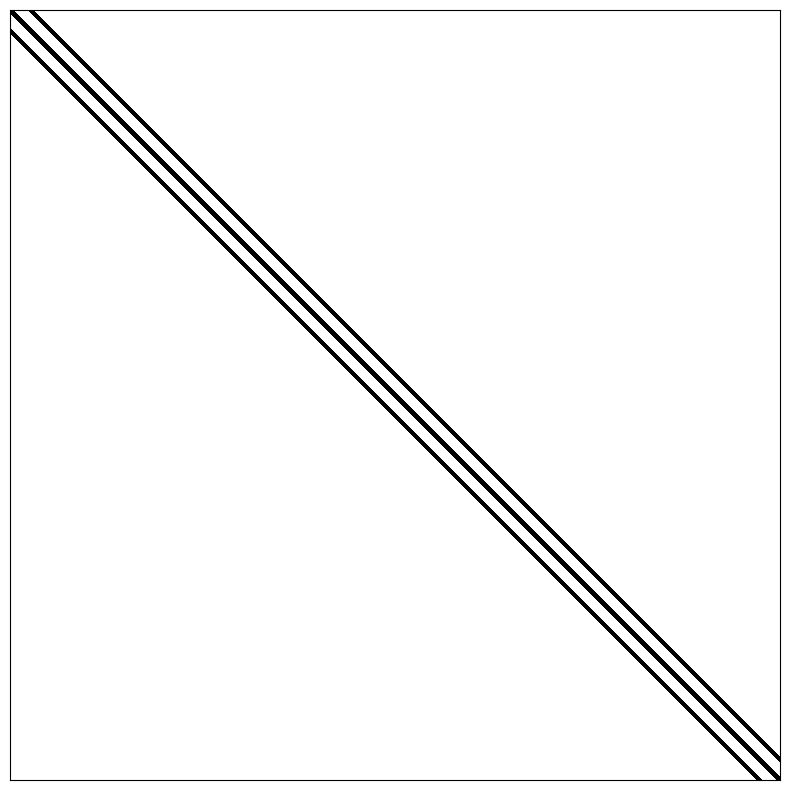
\includegraphics[width=.2\linewidth]{img_mtx_atmosmodm-crop.png}  &
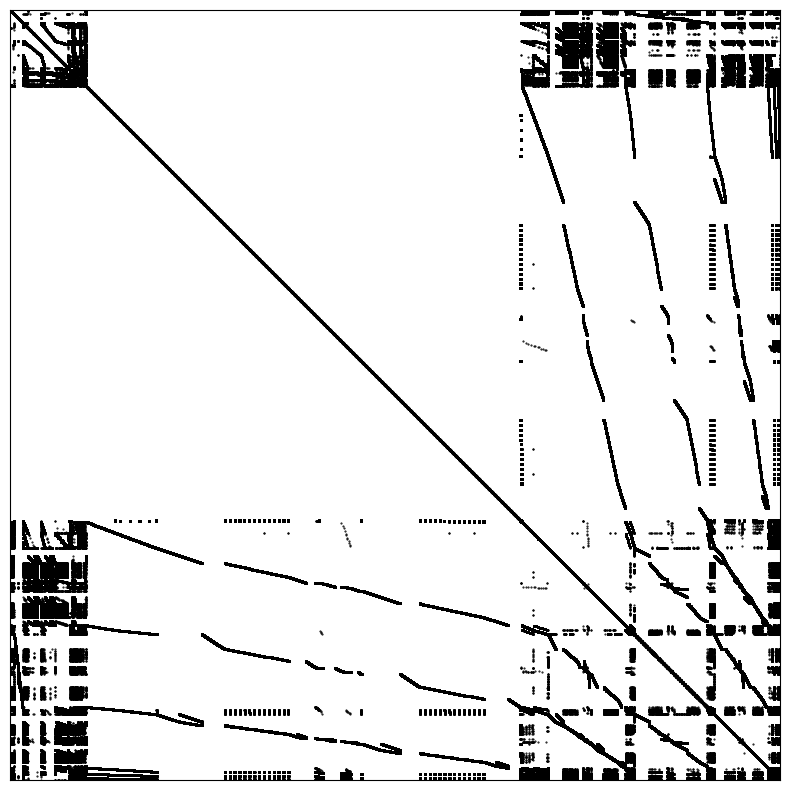
\includegraphics[width=.2\linewidth]{img_mtx_Freescale1-crop.png}  &
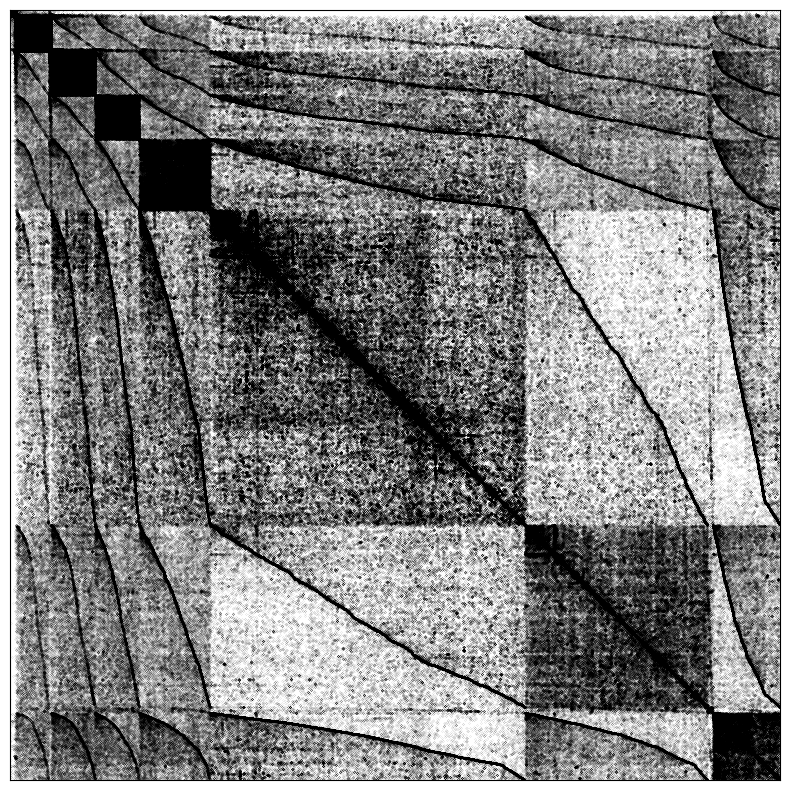
\includegraphics[width=.2\linewidth]{img_mtx_great-britain_osm-crop.png}  &
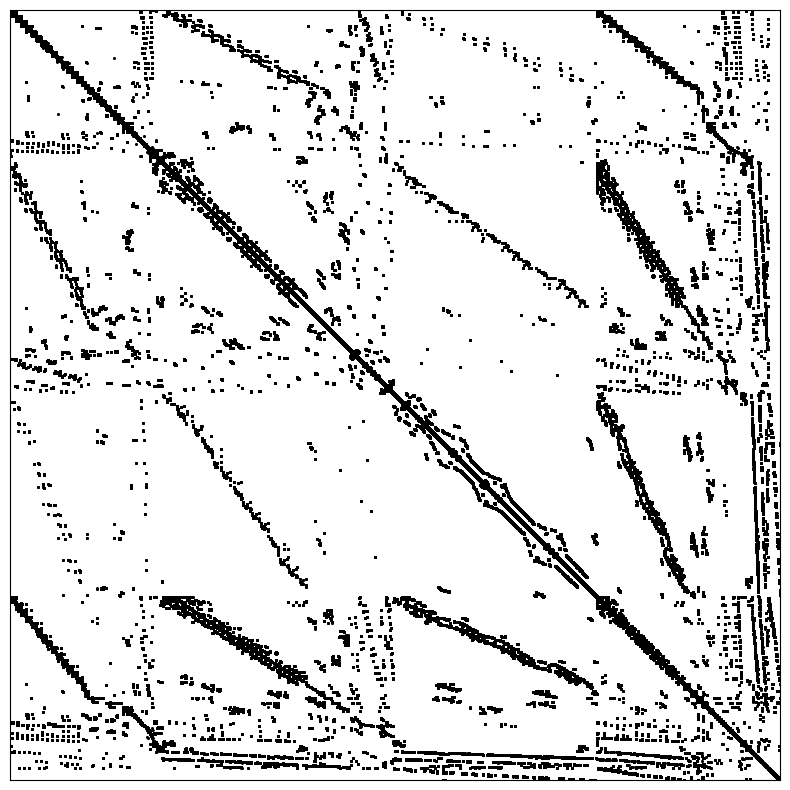
\includegraphics[width=.2\linewidth]{img_mtx_halfb-crop.png}  &
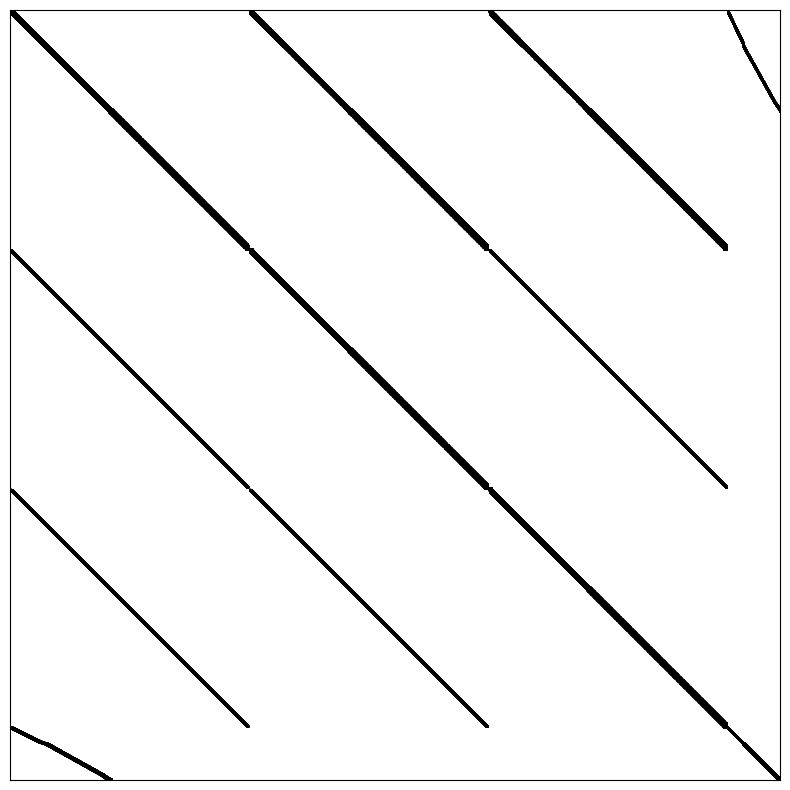
\includegraphics[width=.2\linewidth]{img_mtx_test1-crop.png} \\
\bottomrule
\end{tabular}
}
\end{table}
